
\begin{figure}
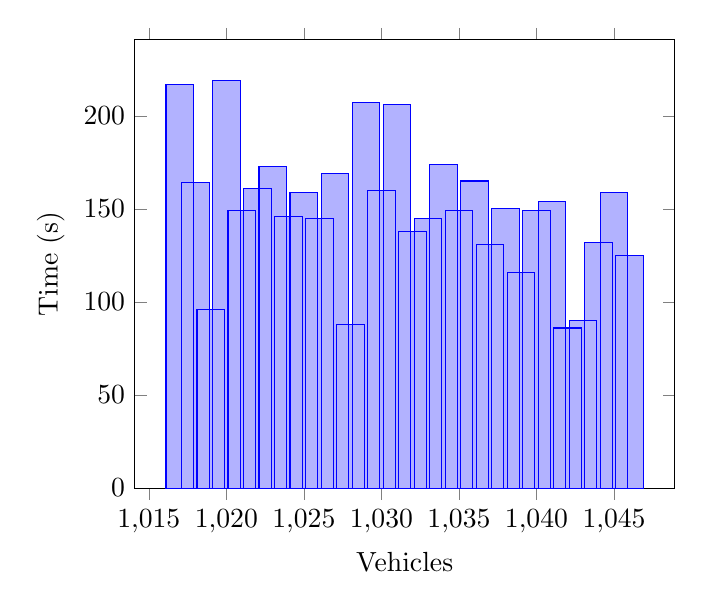
\begin{tikzpicture}
\begin{axis}[
legend style={anchor=west},
xlabel=Vehicles,
ylabel=Time (s),
ymin=0,
ybar,
]
\addplot coordinates {
(1017, 217)
(1028, 88)
(1018, 164)
(1043, 90)
(1042, 86)
(1041, 154)
(1040, 149)
(1046, 125)
(1045, 159)
(1044, 132)
(1019, 96)
(1023, 173)
(1022, 161)
(1032, 138)
(1030, 160)
(1036, 165)
(1037, 131)
(1039, 116)
(1033, 145)
(1031, 206)
(1038, 150)
(1025, 159)
(1024, 146)
(1027, 169)
(1026, 145)
(1021, 149)
(1020, 219)
(1029, 207)
(1034, 174)
(1035, 149)
};

\end{axis}
\end{tikzpicture}
\label{tik:time:0:96}
\caption{0 percent diving with GSC on route $96$}
\end{figure}
